%!TEX root = /Users/markelikalderon/Documents/Git/formwithoutmatter/aristotle.tex
\chapter{Form Without Matter} % (fold)
\label{cha:form_without_matter}

The doctrine that perception involves the assimilation of sensible form without matter is explained in terms of an analogy with the impression made upon wax by a signet ring:
\begin{quote}
	Generally, about all perception, we can say that a sense is what has the power of receiving into itself the sensible forms of things without the matter, in the way in which a piece of wax takes on the impress of a signet-ring without the iron or gold; what produces the impression is a signet of bronze or gold, but not qua bronze or gold: in a similar way the sense is affected by what is coloured or flavoured or sounding not insofar as each is what it is, but insofar as it is of such and such a sort and according to its form. (\emph{De Anima} \textsc{ii}.12 424\( ^{a} \)18--23; Smith in \citealt[42--43]{Barnes:1984uq})
\end{quote}

The analogy is, of course, of Platonic provenance. In the \emph{Theaetetus}, Plato writes;
\begin{quotation}
	\textsc{socrates}: You will think better of it when you hear the rest. To judge truly is a fine thing and there is something discreditable in error.
	
	\textsc{theaetetus}: Of course.
	
	\textsc{socrates}: Well, they say the differences arise in this way. When a man has in his mind a good thick clab of wax, smooth and knealed to the right consistency, and the impressions that come through the senses are stamped on these tables of the `heart'---Homer's words hints at the mind's likeness to wax---then the imprints are clear and deep enough to last a long time. Such people are quick to learn and also have good memories, and besides they do not interchange the imprints of their perceptions but think truly. These imprints being distinct and well spaced are quickly assigned to their several stamps---the `real things' as they are called---and such men are said to be clever. Do you agree?
	
	\textsc{theaetetus}: Most emphatically.
	
	\textsc{socrates}: When a person has what the poet's wisdom commends as a `shaggy heart', or when the block is muddy or made of impure wax, or oversoft or hard, the people with soft wax are quick to learn, but forgetful, those with hard wax, the reverse. Where it is shaggy or rough, a gritty kind of stuff containing a lot of earth or dirt, the impressions obtained are indistinct; so are they too when the stuff is hard, for they have no depth. Impressions in soft wax also are indistinct, because they melt together and soon become blurred. And if besides this, they overlap through being crowded together into some wretched little narrow mind, they are still indistinct. All these types are likely to judge falsely. When they see or hear or think of something, they cannot quickly assign things to their several imprints. Because they are so slow and sort things into their wrong places, they constantly see and hear and think amiss, and say they are mistaken about things and stupid. (Plato, \emph{Theaetetus} 194\( ^{c} \)--195\( ^{a} \); Cornford in \citealt{Hamilton:1961fk})
\end{quotation}

One salient difference between the Aristotelian and Platonic analogies is that whereas Aristotle deploys the wax analogy to explain perception, Plato does so to explain judgment. This difference is most likely intentional and pointed. As we discussed in chapters~\ref{sec:definition} and \ref{sec:the_objects_of_perception}, and as \citet{Sorabji:1971fr,Sorabji:2003fk} emphasizes, Aristotle is extending the domain of perception as Plato conceives of it. Not only are the objects of perception no longer confined to the primary objects---we perceive common sensibles as well---but Aristotle also maintains that we can discriminate among sensory objects and this is the exercise of our perceptual capacities. Plato, in contrast, maintained that what is ``common'' to the objects of sense---that they are each the same and different from the others---is determined by cognitive, not perceptual capacities. Aristotle underscores this extension of our perceptual capacities by using the analogy that Plato used to explain judgment to explain perception instead.

Not only does Aristotle deploy the Platonic analogy to explain his conception of perception, but he also transforms the significance of that analogy. Plato's explanation of the reliability of memory and judgment crucially relies on causal features of the situation. An objects' impression is the effect it has on the mind's wax. Importantly, however, Aristotle has in mind a non-causal sense of impression.

To get a sense of this, first consider how Hume himself appropriates the Platonic analogy:
\begin{quote}
	All the perceptions of the human mind revolves themselves into two distinct kinds, which I shall call \textsc{impressions} and \textsc{ideas}. The difference betwixt these consists in the degree of force or liveliness, with which they strike upon the mind, and make their way into thought and consciousness. (Hume, \emph{Treatise} \textsc{i}.1.1.1)
\end{quote}
Hume begs his reader's indulgence in taking liberty with the use of the terms ``impression'' and ``idea'' (\emph{Treatise} \textsc{i}.1.1 n2) though he proclaims that it is at least a virtue of his regimentation that he ``restore[s] the word, \emph{idea}, to its original sense, from which Mr. \emph{Locke} had perverted it, in making it stand for all our perceptions.'' Hume is presumably taking liberty with his use of the term ``perception'' as well. Locke perverts the use of ``idea'' by making it stand for all perceptions. But perception, here, is not confined to the objects of sensory experience. By ``perception'' Hume means whatever is or could be the object of the mind (admittedly in a post-Cartesian conception of mind unavailable to the ancients). The perceptions present to the human mind are either impressions or ideas, depending upon the force or liveliness with which they strike the mind. Impressions are the objects that are presented with ``the most force and violence'' (\emph{Treatise} \textsc{i}.1.1.1).  Concerning impressions, Hume further explains:
\begin{quote}
	By the term \emph{impression} I wou'd not be understood to express the manner, in which our lively perceptions are produc'd in the soul, but merely the perceptions themselves; for which there is no particular name either in \emph{English} or any other language, that I know of. (\emph{Treatise}, \textsc{i}.1.1 n2)
\end{quote}
Consistent with this qualification, Hume is nevertheless operating with a causal notion of impression. The lively perceptions present before the mind in viewing the streets of Edinburgh are themselves the effect of external causes. However, inquiring after the manner in which such lively perceptions are produced in the soul does not fall within the purview of Hume's new science of human nature but rather belongs to a particular branch of natural philosophy, speculative anatomy. The qualification does not deny that impressions are effects. It rather signals Hume's intention to confine himself to what might be described in a later terminology as the phenomenological objects of consciousness.

So Hume is still thinking of impressions as the effects produced in the perceiver by external objects acting upon them. How else might talk of impressions be understood? 

Consider the related metaphor of shaping. There is clearly a causal sense of shaping. When the signet ring shapes the wax it causes the wax to be modified in a certain way. The wax takes on the shape imposed upon it by the signet ring. Similarly, Nazi bombing shaped the London skyline. It caused that skyline to be configured in a certain way, the way imposed upon it by the bombing. Importantly, however, there is another sense of shaping, not a causal sense but a constitutive sense. Whereas Nazi bombing shaped the London skyline in a mere causal sense, St Paul's constitutively shapes that skyline by being a contour of that skyline (as in Herbert Mason's iconic photograph see figure~\ref{fig:stpauls}).

\begin{figure}[htbp]
	\centering
		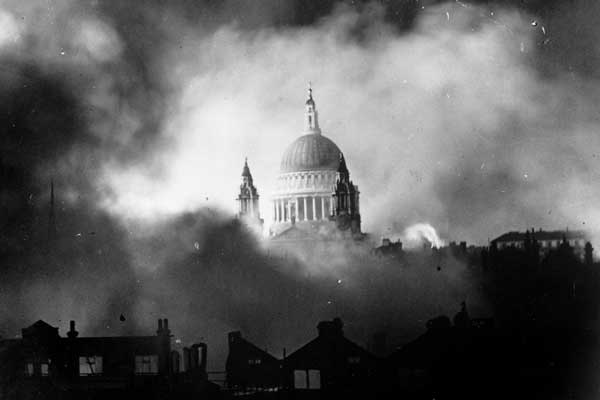
\includegraphics[scale=0.6]{graphics/stpauls.jpg}
	\caption{St Paul's 29 December 1940}
	\label{fig:stpauls}
\end{figure}

Humean sensory impressions are shaped by the environment merely in a causal sense. This is central to Hume's use of the Platonic analogy. Just as a signet ring impinging upon the wax causes an impression, the environment impinging upon a perceiver with the appropriate sensory capacities causes a sensory impression. But perhaps perceptual sensitivity is more than the environment impinging upon the state of a conscious subject. Perhaps there is more to perception than objects eliciting a conscious modification of the perceiving subject. Perhaps the environment can shape sensory consciousness in a constitutive rather than merely a causal sense.

Before exploring this idea further, let us first consider one further aspect of the Platonic analogy. Caston makes the important observation that the impression produced by a signet ring is linked to that particular ring and, hence, metonymically, to the legitimate possessor of that ring:
\begin{quote}
	A signet produces a sealing, an impression that establishes the identity of its owner and consequently his authority, rights, and prerogatives. When a sealing is placed on a document, especially for legal or official use, it authorizes the claims, obligations, promises, or orders made therein. A sealing thus differs from other impressions in that it \emph{purports to originate from a particular signet}. \citep[302]{Caston:2005cr}
\end{quote}

% chapter form_without_matter (end)
